\clearpage
\section{RX-side Image Rejection}
\label{sec:rx-image-rejection}

\textbf{A Motivating Example.} Image rejection is one of those receiver concepts that rarely clicks the first
time it's explained in the abstract, so start with concrete numbers instead of the general formula. Suppose we
want to receive an RF signal on FR3 at 15\,GHz, downconverted to a 2\,GHz FR1 IF output, using a high-side LO at
17\,GHz (LO = FR3 + FR1). The mixer only computes |RF − LO|, so it faithfully
turns our desired 15\,GHz input into the 2\,GHz output we want: |15 − 17| = 2\,GHz. Now suppose the antenna also
picks up some unrelated transmission at 19\,GHz --- a different system entirely, with nothing to do with the
signal we're trying to receive. That 19\,GHz \emph{also} satisfies |RF − LO| = |19 − 17| = 2\,GHz,
so it also downconverts to exactly 2\,GHz, landing right on top of the signal we actually want. Nothing after
the mixer can tell which part of that 2\,GHz output came from the real 15\,GHz transmission and which came from
the unrelated 19\,GHz one --- they are now the same signal. The 19\,GHz frequency here is the \emph{image}. Our
goal is to reject as much of the image (19\,GHz) as possible while keeping as much of the desired signal
(15\,GHz) as possible --- that is image rejection.

\textbf{What's plotted.} The example above generalizes directly for a down-converting mixer: for any LO and any
IF, there are always two RF input frequencies, LO + IF and LO − IF, that produce
that same output IF, sitting the same distance from the LO but on opposite sides of it; whichever one isn't the
signal we intend to receive is called the undesired \emph{image}. This section measures how well this unit
rejects it.\footnote{Every point here is one real CW-tone measurement, not an average over a swept window.} The
image, in real operation, is never something this unit's own receiver produced --- it is whatever else happens
to be transmitting in that unrelated band at that moment. Testing image rejection is quite simple: (1) feed in
an RF tone at LO + IF and measure the IF output, then (2) feed in an RF tone at
LO − IF and measure the IF output. One of these is desired and the other is undesired, depending
on whether we are using high-side or low-side LO. The ratio of the desired to undesired power values
(difference, since we're calculating in dB) is the image rejection. The Pi-Radio unit rejects the unwanted
signal by simply filtering the input RF signal using the AM3153 filter before it ever hits the mixer.

\textbf{Why rejection comes from the filter alone.} The AM3153 tracking filter sits before the mixer in the RX
chain (LNA → AM3153 → mixer), so it acts as an RF pre-select filter that attenuates the image frequency
before it ever reaches the mixer --- the classic filter-based image-rejection technique, and the \emph{only}
image-rejection mechanism this side of the board has.\footnote{The same AM3153 already in the chain for band
selection does double duty as the image-reject filter --- there is no separate, dedicated image-reject
component.} The bypass figures show what happens with no filter at all, the same honest baseline convention
used in Section~\ref{sec:sideband-suppression}; the optimal figures use the same ``optimal'' filter-selection
algorithm described there, re-applied here for RX.

\textbf{Measurement conditions.} CW tones at −50\,dBm into the ``RX-side FR3 RF In'' connector, first at the desired frequency, then at the image; otherwise as in Section~\ref{sec:rx-gain-lowside}. LMX2820 die at \condRxImageMinC--\condRxImageMaxC\textdegree C.

\textbf{When does image rejection matter?} Suppose we're trying to receive an RF signal at LO $\pm$ IF. Image
rejection matters only when there is an interferer transmitting at LO $\mp$ IF; otherwise, it doesn't matter. If
such an interferer is known to exist for the current
configuration (high-side or low-side LO), then switch to the other configuration (low-side or high-side LO).
This moves the location of the LO and also the undesired image, thereby mitigating the interference. From
Figures~\ref{fig:11-1} and~\ref{fig:11-5}, observe that if the filter is not engaged, image rejection is poor.
However, engaging the optimal filter (Figures~\ref{fig:11-3} and~\ref{fig:11-7}) helps a lot with image
rejection.\footnote{Two points in the low-side grid (LO~=~7\,GHz, IF~=~3.5\,GHz, and LO~=~8\,GHz, IF~=~4.0\,GHz
--- the only two points satisfying LO = 2×IF) show anomalously poor image rejection despite excellent rejection at every neighboring point, visible in Figure~\ref{fig:11-3}. This was
confirmed to be a real hardware effect rather than a measurement error: reproduced across repeated,
independently re-locked measurements. Through offset measurements, we diagnosed the cause to be the
(3·RF - LO) spur leaking in when the \emph{undesired image} was fed as the input. Avoiding
this spur is simple: (1) avoid configurations where 2×IF = LO; or (2) choose the sideband
so as to keep the LO at 9\,GHz or above.}\xdef\imgrejoutlierfn{\therealfootnote}% footnote number, for the callout on the optimal-filter heatmap
 Observe that even with the filter engaged, image rejection is poorer at low IF frequencies; this is
because the desired and undesired images are very close together, making it harder for the filter to get rid of
the unwanted image. To mitigate this, operate the system at a higher IF (FR1) frequency for the same incoming RF
signal; this gives the filter more headroom to filter out the interferer.

\textbf{Could we have achieved better image rejection?} In the current hardware, the mixer produces the IF
outputs in quadrature; we discard Q and keep I, since both carry identical information. However, had we passed
this through a 90$^\circ$ hybrid coupler (with a DPDT switch to achieve I/Q through or swap, like we did on the
TX side), the image rejection would have improved further. We plan to do this in a future hardware revision.

\clearpage
% Tighter, section-local figpair: all 4 rows (8 figures) must fit on one page together (see the
% "When does image rejection matter?" paragraph above, which refers to all of them by number). Scoped to
% this \begingroup/\endgroup block so the document-wide \figpair spacing is untouched elsewhere.
\begingroup
\renewcommand{\figpair}[6]{%
  \noindent
  \begin{minipage}[t]{0.46\linewidth}
    \centering
    \includegraphics[width=\linewidth]{#1}
    \captionof{figure}{#2}\label{#3}
  \end{minipage}\hfill
  \begin{minipage}[t]{0.46\linewidth}
    \centering
    \includegraphics[width=\linewidth]{#4}
    \captionof{figure}{#5}\label{#6}
  \end{minipage}
  \par\vspace{0.3em}
}
\figpair{images/sec11_fig1.pdf}{LO: Low-side. Filter: Bypassed. Image rejection (dB) across the full grid.}{fig:11-1}%
        {images/sec11_fig2.pdf}{LO: Low-side. Filter: Bypassed. Distribution of Figure~\ref{fig:11-1}.}{fig:11-2}
% Same layout as the local \figpair above, but the left panel carries a TikZ overlay: red circles around the two
% LO = 2 x IF outliers at (FR1, FR3) = (3.5, 10.5) and (4.0, 12.0) GHz, and a callout whose footnote number is
% taken from the footnote itself (\imgrejoutlierfn), so it can't go stale. Positions are fractions of the image
% width/height, measured from the figure's axis ticks.
\noindent
\begin{minipage}[t]{0.46\linewidth}
  \centering
  \begin{tikzpicture}
    \node[anchor=south west, inner sep=0] (img) at (0,0) {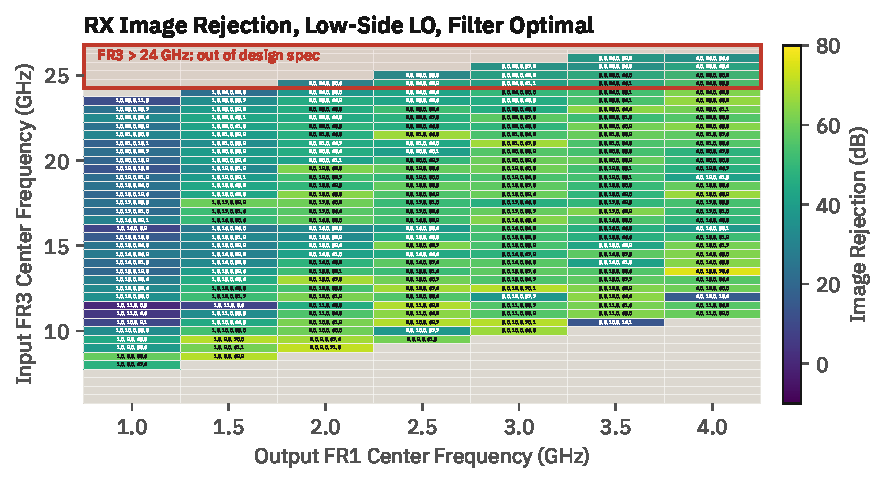
\includegraphics[width=\linewidth]{images/sec11_fig3.pdf}};
    \begin{scope}[x={(img.south east)}, y={(img.north west)}]
      \draw[red!80!black, line width=0.9pt] (\imgOutlierAX,\imgOutlierAY) circle (4.2pt);
      \draw[red!80!black, line width=0.9pt] (\imgOutlierBX,\imgOutlierBY) circle (4.2pt);
      \node[red!80!black, font=\tiny\bfseries, anchor=north] at ({(\imgOutlierAX+\imgOutlierBX)/2},{\imgOutlierAY-0.03}) {See footnote \imgrejoutlierfn};
    \end{scope}
  \end{tikzpicture}
  \captionof{figure}{LO: Low-side. Filter: Optimal. Image rejection (dB) across the full grid.}\label{fig:11-3}
\end{minipage}\hfill
\begin{minipage}[t]{0.46\linewidth}
  \centering
  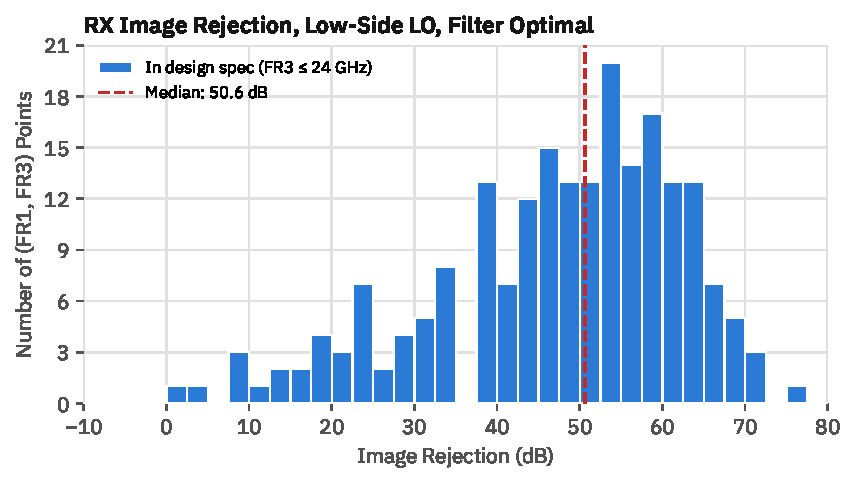
\includegraphics[width=\linewidth]{images/sec11_fig4.pdf}
  \captionof{figure}{LO: Low-side. Filter: Optimal. Distribution of Figure~\ref{fig:11-3}.}\label{fig:11-4}
\end{minipage}
\par\vspace{0.3em}
\figpair{images/sec11_fig5.pdf}{LO: High-side. Filter: Bypassed. Image rejection (dB) across the full grid.}{fig:11-5}%
        {images/sec11_fig6.pdf}{LO: High-side. Filter: Bypassed. Distribution of Figure~\ref{fig:11-5}.}{fig:11-6}
\figpair{images/sec11_fig7.pdf}{LO: High-side. Filter: Optimal. Image rejection (dB) across the full grid.}{fig:11-7}%
        {images/sec11_fig8.pdf}{LO: High-side. Filter: Optimal. Distribution of Figure~\ref{fig:11-7}.}{fig:11-8}
\endgroup
